\chapter{Opis problemu}
\section{Rozmiar i ukad treci na stronach dokumentu}
Praca dyplomowa powinna by przygotowana do wydruku na papierze formatu A4 w orientacji pionowej.
Marginesy na stronach parzystych i nieparzystych powinny by jednakowe i mie nastpujce wartoci:
lewy = 25mm, prawy = 25mm, grny = 10mm, dolny = 15mm. Wielko marginesw w szablonie sterowana jest parametrami przedstawionymi na rysunku~\ref{fig:pageLayout}. Margines dolny powinien by mierzony do linii bazowej tekstu stopki.
%\begin{figure}[htb]
	%\centering
	%\includegraphics[width=.7\linewidth]{rys03/pageLayout2}
	%\caption{Kontrola marginesw i odstpw elementw na stronie} \label{fig:pageLayout}
%\end{figure}
\begin{figure}[htb]
\setlayoutscale{0.43}
\currentpage
\drawparameterstrue
%\drawpage
\oddpagelayoutfalse
\drawstock
\caption{Ukad strony nieparzystej dla dokumentu klasy \texttt{memoir}} \label{fig:pageLayout}
\end{figure}

Rzeczywisty ukad strony zastosowany w niniejszym dokumencie przedstawiono na rysunku~\ref{fig:currentPageLayout}. Lewy i prawy margines s takie same, wic strony parzyste i nieparzyste wygldaj podobnie, z dokadnoci do umiejscowienia notatek marginesowych. Taki rezultat zapewnio zastosowanie poniszych komend. 
\begin{figure}[t]
\setlayoutscale{0.43}
\currentstock
\oddpagelayouttrue
\twocolumnlayoutfalse
\drawmarginparstrue
\drawparametersfalse
\drawstock
\caption{Rzeczywisty ukad strony nieparzystej w tym dokumencie} \label{fig:currentPageLayout}
\end{figure}

\begin{lstlisting}[basicstyle=\footnotesize\ttfamily]
\setlength{\headsep}{10pt} 
\setlength{\headheight}{13.6pt} 
\setlength{\footskip}{\headsep+\headheight}
\setlength{\uppermargin}{\headheight+\headsep+1cm}
\setlength{\textheight}{\paperheight-\uppermargin-\footskip-1.5cm}
\setlength{\textwidth}{\paperwidth-5cm}
\setlength{\spinemargin}{2.5cm}
\setlength{\foremargin}{2.5cm}
\setlength{\marginparsep}{2mm}
\setlength{\marginparwidth}{2.3mm}
\checkandfixthelayout[fixed] 
\linespread{1}
\setlength{\parindent}{14.5pt}
\end{lstlisting}




\section{Strona tytuowa}
Wedug oglnouczelnianych zalece (tj.\ logotypu Politechniki Wrocawskiej) strona tytuowa powinna by zredagowana z~uyciem czcionki \texttt{garamond}. W oficjalnym wzorcu (patrz rysunek~\ref{fig:stronaTytulowa})
nie rozrniono, czy dotyczy on pracy inynierskiej czy magisterskiej. 
\begin{figure}[b]
	\centering
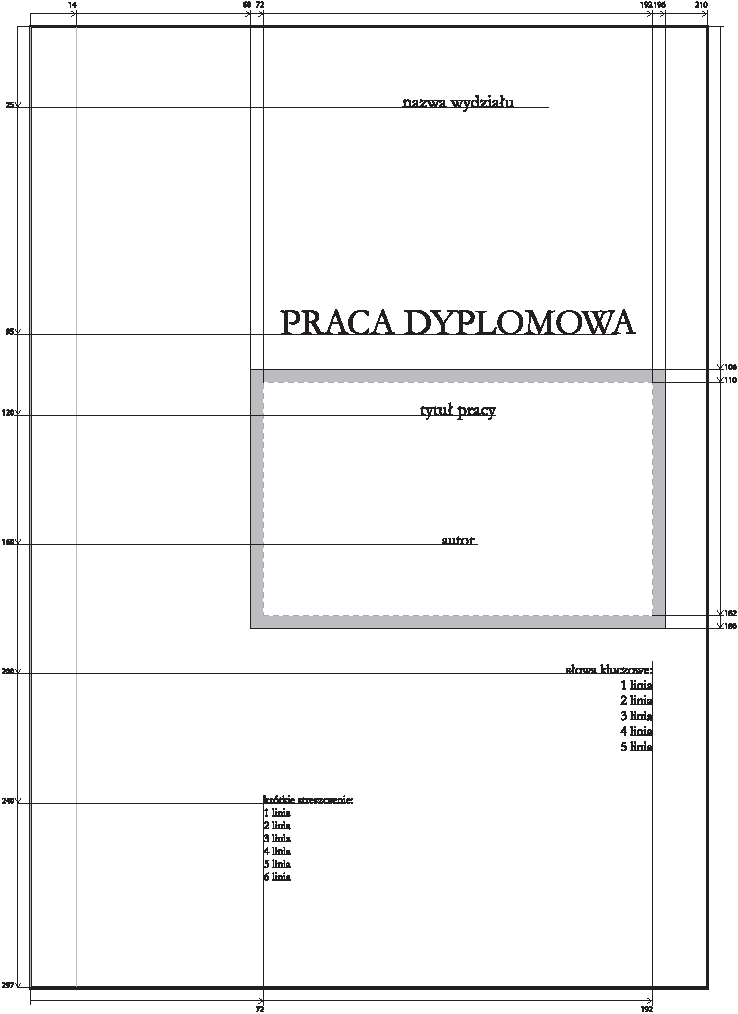
\includegraphics[width=.6\linewidth]{rys03/stronaTytulowa01}
	\caption{Oficjalny szablon strony tytuowej pracy dyplomowej, zamieszczony w dokumencie ,,System 
Identyfikacji Wizualnej Wrocaw, sierpie 2016'' do pobrania ze strony \url{http://pwr.edu.pl/uczelnia/o-politechnice/materialy-promocyjne/logotyp} [dostp dnia 07.12.2016]}
	\label{fig:stronaTytulowa}
\end{figure}
Nie uwzgldniono rwnie miejsca na nazw specjalnoci ani kierunku oraz zapomniano o nazwisku promotora, jednostce, dacie i ocenie.  Za to okrelono (zgrubnie) pooenie sw kluczowych i~streszczenia. Poniewa brakujce dane pojawiay si we wzorcach stron tytuowych stosowanych w~codziennej praktyce na Wydziaach, nie wiadomo do koca, czy oficjalny szablon naley stosowa w 100 procentach. Dlatego w niniejszym dokumencie zastosowano wasny wzorzec strony tytuowej (uywany od lat) oraz podano wymagania odnonie wzorca z~logotypu uczelnianego.

Wymagania co do wielkoci znakw na stronie tytuowej s nastpujce:
\begin{itemize}
\item wedug uczelnianego logotypu
\begin{lstlisting}[basicstyle=\footnotesize\ttfamily]
Nazwa jednostki organizacyjnej: Garamond 16 pt 
Napis "PRACA DYPLOMOWA INYNIERSKA": Garamond 32 pt 
Tytu pracy: Garamond 16 pt 
Autor: Garamond 14 pt 
Sowa kluczowe: Garamond 12 pt 
Krtkie streszczenie: Garamond 10 pt 
\end{lstlisting}
\item wedug wzorca uytego w niniejszym dokumencie
\begin{lstlisting}[basicstyle=\footnotesize\ttfamily]
POLITECHNIKA WROCAWSKA (Garamond 22pt 24pt)
WYDZIA ELEKTRONIKI (Garamond 22pt 24pt)
KIERUNEK: JAKI KIERUNEK (Garamond 14pt 16pt)
SPECJALNO: JAKA SPECJALNO (Garamond 14pt 16pt)
PRACA DYPLOMOWA (Garamond 24pt 26pt)
INYNIERSKA (Garamond 24pt 26pt)
Tytu pracy w jzyku polskim (Garamond 16pt 18pt)
Title in English (Garamond 16pt 18pt)
AUTOR: (Garamond 16pt 18pt)
Imi Nazwisko (Garamond 14pt 16pt)
PROWADZCY PRAC: (Garamond 16pt 18pt)
tytu, Imi Nazwisko, Jednostka (Garamond 14pt 16pt)
OCENA PRACY: (Garamond 16pt 18pt)
WROCAW, 2015 (Garamond 16pt 18pt)
\end{lstlisting}
\end{itemize}

W szablonie zastosowano pakiet \texttt{ebgaramond}. Dostarcza on klonu czcionki \texttt{garamond}, jednak bez ksztatu \texttt{slanted} i z pewnymi brakami. Na przykad zamiast literki ,,'' w zbiorze \texttt{EBGaramond08 Italic} renderuje si samo ,,l'' (braku tego nie ma zbir \texttt{EBGaramond12}).  Zalet pakietu  w porwnaniu do innych jest to, e generalnie dobrze obsugiwane s w nim polskie znaki oraz e pakiet ten mona znale w rnych dystrybucjach latexa (\texttt{MikTeX} instaluje go automatycznie).

\section{Krj i wielko czcionek}
Gwny tekst pracy powinien by zredagowany z wykorzystaniem czcionki \texttt{Times}, typ normalny, o wysokoci 12pt, z odstpem midzy liniami rwnym 14.5pt. Istnieje moliwo zmiany odstpu midzy liniami za pomoc komendy \verb?\linespread?, jednak zaleca si pozostawienie tego odstpu jak w niniejszym dokumencie (\verb?\linespread{1}?). Wymagania odnonie kroju pisma pozostaych elementw (nagwkw, stopek itp.) zamieszczono w tabeli~\ref{tab:secfonts}.

W szablonie zastosowano czcionk \texttt{texgyre-termes} (dostarcza j pakiet \texttt{tgtermes}). Czcionka ta jest klonem czcionki \texttt{Times}, w ktrym obsugiwane jest rodkowoeuropejskie kodowanie znakw (podobnie jak w przypadku czcionki \texttt{ebgaramond}, dziki czemu polskie literki nie s zlepkami dwch znakw lecz pojedynczymi znakami).  

Wszelkie przykady rde kodu (fragmenty programw, komendy linii polece), nazwy plikw i uruchamianych programw powinny by pisane czcionk maszynow. W szablonie czcionk maszynow jest \texttt{t1xtt}. Czcionka ta obsuguje polskie znaki. Dostarcza j pakiet \texttt{txfonts}, ktry naley wczeniej zainstalowa (MiKTeX zainstaluje go automatycznie podczas pierwszej kompilacji szablonu).   

% https://en.wikibooks.org/wiki/LaTeX/Lengths
% there are two different point sizes.  A pdf point is 1/72 inch.  A LaTeX point is 1/72.27 inch.  Thus,
% the LaTeX point is slightly smaller than a pdf point. 

%\texttt{baselineskip}: \printlength{\baselineskip}\\
%\texttt{beforesecskip}: \printlength{\beforesecskip}\\
%\texttt{aftersecskip}: \printlength{\aftersecskip}\\
%\texttt{topskip}: \printlength{\topskip}\\
%\texttt{fontsize}: \showFontSize\\

\begin{table}[htb]
\centering
\caption{Zestawienie czcionek elementw podziau dokumentu, tekstu wiodcego, nagwka i stopki oraz podpisw (Rozm. -- rozmiar czcionki, Odst. -- \texttt{baselineskip})}
\label{tab:secfonts}\small
\begin{tabularx}{\linewidth}{|ll@{\hskip 5pt}l@{\hskip 5pt}lX|} \hline
Element & Przykad & Czcionka & Rozm. & Odst. \\ \hline\hline
Nr rozdziau & {\huge\bfseries Rozdzia 1 } & \verb?\huge\bfseries? & 25pt & 30pt \\
Tytu rozdziau & {\Huge\bfseries Wstp } & \verb?\Huge\bfseries? & 30pt & 37pt\\
Nr i tytu sekcji & {\Large\bfseries 1.1. Wprowadzenie } & \verb?\Large\bfseries? & 17pt & 22pt \\
Nr i tytu podsekcji & {\large\bfseries 1.1.1. Cel szczegowy } & \verb?\large\bfseries? &14.5pt & 18pt\\
Tytu podpodsekcji  & {\normalsize\bfseries Zaoenia } & \verb?\normalsize\bfseries? & 12pt & 14.5pt\\
Tytu paragrafu & {\normalsize\bfseries  Podstawy } Opis ... &  \verb?\normalsize\bfseries? & 12pt & 14.5pt\\
Tekst wiodcy & {\normalsize Niniejszy dokument ... } & \verb?\normalsize? & 12pt & 14.5pt\\
Nagwek strony & {\small\itshape 3.2. Czcionka wiodca ...} & \verb?\small\itshape? & 11pt & 13.6pt \\
Stopka strony & {\small Imi Nazwisko: ...} & \verb?\small? & 11pt & 13.6pt\\
Podpisy tabel & {\small Tab.~3.1: Zestawienie ...} & \verb?\small? & 11pt & 13.6pt \\
Podpisy rysunkw & {\small Rys.~3.1: Oficjalny ...} & \verb?\small? & 11pt & 13.6pt\\\hline
\end{tabularx}
\end{table}
%\texttt{fontsize}: \showFontSize

Jeli w pracy zostan uyte otoczenia matematyczne, to w dokumencie wynikowym pojawi si dodatkowe czcionki (domylne latexowe czcionki do wyrae matematycznych). Dziki zastosowaniu opcji \texttt{extrafontsizes} w klasie \texttt{memoir} nie do, e otrzymuje si wiksze czcionki (30pt), to jeszcze zamiast \texttt{Computer Modern} do wzorw matematycznych jest stosowana czcionka \texttt{Latin Modern} (wywodzca si z \texttt{Computer Modern}).
Std lista wszystkich uytych czcionek moe by nastpujca:
\begin{lstlisting}[basicstyle=\footnotesize\ttfamily]
EBGaramond12-Regular
GaramondNo8-Reg-Norml
TeXGyreTermes-Regular-Normalna
TeXGyreTermes-Bold-Pogrubiona
TeXGyreTermes-Italic-Normalna
t1xtt-Nomal
LMMathItalic12-Regular
LMMathSymbols10-Regular
LMMathExtension10-Regular
LMRoman8-Regular
\end{lstlisting}

Aby wykorzysta te czcionki poza systemem LaTeX, wystarczy pobra je spod adresw (wanych na dzie
1.04.2016): 
\url{https://www.ctan.org/tex-archive/fonts/cm/ps-type1/bakoma/ttf/?lang=en}, \url{http://www.gust.org.pl/projects/e-foundry/latin-modern}, \url{http://www.gust.org.pl/projects/e-foundry/tex-gyre}, \url{https://bitbucket.org/georgd/eb-garamond/downloads},
a nastpnie zainstalowa w systemie. Dziki temu mona bdzie np.~edytowa rysunki uywajc dokadnie tej samej czcionki, co czcionka uyta w dokumencie.

\section{Formatowanie blokw tekstu}
Kady rozdzia pracy powinien rozpoczyna si od nowej strony. Jej wygld powinien by kontrolowany parametrami pokazanymi na rysunku~\ref{fig:LayChap}.
\begin{figure}[t]
\setlayoutscale{0.7}
\centering
\chapterdiagram
\caption{Parametry sterujce wielkociami odstpw na stronie z tytuem rozdziau} 
\label{fig:LayChap}
\end{figure}
W niniejszym szablonie (dokument klasy \texttt{memoir} z opcj \texttt{[12pt]}) przyjto nastpujce wartoci tych parametrw:
\begin{itemize}
\item \verb?\beforechapskip? (\printlength{\beforechapskip}) + \verb?\baselineskip? of \verb+\huge+ (30pt) + \verb+\topskip+ (\printlength{\topskip}) = 92pt (3.246cm)
\item \verb?\midchapskip? (\printlength{\midchapskip}) + \verb?\baselineskip? of \verb+\Huge+ (37pt) = 57 pt (2.011cm)
\item \verb?\afterchapskip? (\printlength{\afterchapskip}) + \verb+\baselineskip+ of \verb+\normalsize+ (14.5pt) = 54.5pt (1.923cm)
\end{itemize}

Nieco kopotw moe sprawi dobre ustawienie na stronie tytuw nienumerowanych rozdziaw oraz list generowanych automatycznie (Skrty, Spis treci, Spis rysunkw, Spis tabel, Indeks rzeczowy). W szablonie w tym celu zdefiniowano nowy styl rozdziau komendami jak niej (w szablonie s to komendy zamarkowane)
\begin{lstlisting}[basicstyle=\footnotesize\ttfamily]
\newlength{\linespace}
\setlength{\linespace}{-\beforechapskip-\topskip+\headheight+\topsep}
\makechapterstyle{noNumbered}{%
\renewcommand\chapterheadstart{\vspace*{\linespace}}
}
\end{lstlisting}
oraz dokonano przeczenia stylw rozdziaw komendami \verb?\chapterstyle{nonumbered}? oraz \verb?\chapterstyle{default}? podczas doczania do dokumentu wymienionych nienumerowanych rozdziaw i list. Aby ,,podnie do gry'' tytuy nienumerowanych rozdziaw (gdyby jest to rzeczywicie konieczne) wystarczy odmarkowa wspomniane komendy.

Tytuy rozdziaw, sekcji, podsekcji itd.\ nie powinny koczy si kropk. Odlegoci pomidzy tekstem wiodcym a tytuem sekcji powinien by regulowany parametrami pokazanymi na rysunku~\ref{fig:LaySec}. 
\begin{figure}[t]
%\setlayoutscale{1}
\runinheadfalse
\drawparameterstrue
\drawheading{\Large\bfseries}
\caption{Kontrola ustawie odlegoci w tytuach kolejnych sekcji} 
\label{fig:LaySec}
\end{figure}
Rozmiar \verb?\baselineskip? zaley od rozmiaru czcionki (zobacz tabela~\ref{tab:secfonts}), za \texttt{beforeskip} i \texttt{secskip} od poziomu sekcji. W niniejszym szablonie przyjto nastpujce wartoci tych parametrw (s to wartoci dobierane elastycznie podczas kompilacji):
\begin{itemize}
\item \texttt{indent = 14.5pt}
\item \texttt{parskip = \printlength{\parskip}}
\item \texttt{beforesecskip = \printlength{\beforesecskip}}
\item \texttt{aftersecskip = \printlength{\aftersecskip}}
\item \texttt{beforesubsecskip = \printlength{\beforesubsecskip}}
\item \texttt{aftersubsecskip = \printlength{\aftersubsecskip}}
\item \texttt{beforesubsubsecskip = \printlength{\beforesubsecskip}}
\item \texttt{aftersubsubsecskip = \printlength{\aftersubsecskip}}
\end{itemize}

W szablonie obowizuj rwnie nastpujce wartoci parametrw odpowiedzialnych za odstpy pomidzy pywajcymi figurami, tekstami oraz tekstem i figur:
\begin{itemize}
\item \texttt{floatsep = \printlength{\floatsep}}
\item \texttt{intextsep = \printlength{\intextsep}}
\item \texttt{textfloatsep = \printlength{\textfloatsep}}
\end{itemize}

Pierwsza linia pierwszego akapitu w bloku (po tytule rozdziau, sekcji, podsekcji, podpodsekcji) nie moe mie wcicia. Pierwsze linie w kolejnych akapitach ju powinny mie wcicie rwne 14.5pt. Tekst w akapitach powinien by wyrwnany z obu stron. 


Strony powinny by numerowane numeracj cig (sekwencja arabskich cyfr). Numery stron powinny by umieszczone w ich stopkach (tj. tak jak w niniejszym dokumencie). Wyjtkiem s tutaj pierwsze strony rozdziaw oraz strona tytuowa -- na nich numery nie powinny si pojawi.

W pracy naley dba o poprawno redakcyjn zgodnie z zaleceniami:
\begin{itemize}
\item nie zostawia znaku spacji przed znakami interpunkcji (,,powiedziano , e ...'' -> ,,powiedziano, e ...''),
\item kropki po skrtach, ktre nie s jednoczenie kropkami koczcymi zdanie naley skleja z kolejnym wyrazem znakiem tyldy, np.~jak tutaj (\verb?np.~jak tutaj?) lub wstawia za nimi ukonik, np.\ jak tutaj (\verb?np.\ jak tutaj?)
\item nie zapomina o dobrym sformatowaniu wyliczenia (naley zaczyna maymi literami lub duymi oraz koczy przecinkami, rednikami i kropkami -- w zalenoci od kontekstu danego wyliczenia),
\item nie zostawia samotnych literek na kocach linii  (mona je ,,sklei'' z wyrazem nastpnym stosujc znaczek tilde, jak \verb+w~przykadzie+).
\item nie zostawia pojedynczych wierszy na kocu lub pocztku strony (naley kontrolowa ,,sieroty'' i ,,wdowy''),
\item nie zostawia odstpu pomidzy tekstem a nawiasami czy znakami cudzysoww (znaki te powinny przylega do tekstu, ktry obejmuj ,,jak w tym przykadzie''),
\item wyrazy obcojzyczne powinny by pisane czcionk italic wraz ze skrtem oznaczajcym jzyk, w szczeglnoci ma to zastosowanie przy rozwijaniu skrtw, np.~OGC (ang.~\emph{Open Geospatial Consortium}),
\item kady zastosowany skrt powinien zosta rozwinity podczas pierwszego uycia, pniej moe ju wystpowa bez rozwinicia (skrt i jego rozwinicie powinny trafi rwnie do wykazu Skrty, jeli taki wykaz jest doczany do dokumentu). 
\end{itemize}

\section{Opisy tabel i rysunkw}
Podpisy powinny by umieszczane pod rysunkami lub nad tabelami wraz z etykiet skadajc si ze skrtu Rys.\ lub Tab.\ oraz numeru. Podpisy te nie powinny mie kocowej kropki. Numery wystpujcy w podpisach powinny zaczyna si numerem rozdziau, po ktrym nastpuje kolejny numer rysunku lub tabeli w obrbie rozdziau. Etykieta powinna koczy si dwukropkiem, po ktrym nastpuje tekst podpisu. Numer rozdziau powinien by rozdzielony kropk od kolejnego numeru w rysunku bd tabeli w rozdziale (liczniki tabel i rysunkw s rozczne). Naley pamita o tym, eby w caej pracy tabele miay podobny wygld (rodzaj czcionki, ewentualne pogrubienia w nagwku itp.). %rda naley podawa pod tabel.

\section{Przypisy dolne}
Istnieje moliwo zamieszczania przypisw na dole strony, cho nie jest to zalecane (przykadowo~\footnote{Tekst przypisu}). Sposb parametryzowania ich wygldu pokazano na rysunku~\ref{fig:fp}. W szablonie wykorzystano nastpujce, domylne wartoci tych parametrw:
\begin{lstlisting}[basicstyle=\footnotesize\ttfamily]
\footins = 12pt \footnotesep = 8pt
\baselineskip = 10pt note separation = 40pt
rule thickness = 0.4pt
rule length = 0.25 times the \textwidth
\end{lstlisting}
\begin{figure}[htb]
\setlayoutscale{0.35}
\drawfootnote
\caption{Parametry sterujce przypisami dolnymi} \label{fig:fp}
\end{figure}
%\tryfootins
%\tryfootnotesep
%\tryfootnotebaseline
%\tryfootruleheight
%\tryfootrulefrac

%\footins = 12pt \footnotesep = 8pt
%\baselineskip = 10pt note separation = 40pt
%rule thickness = 0.4pt
%rule length = 0.25 times the \textwidth

\section{Formatowanie spisu treci}
W klasie memoir istniej komendy pozwalajce do dobrze zarzdza wygldem spisu treci. Na rysunku~\ref{fig:ltoc} pokazano, za pomoc jakich parametrw mona wpywa na finaln jego posta. W szablonie wykorzystano nastpujce, domylne ich wartoci:
\begin{lstlisting}[basicstyle=\footnotesize\ttfamily]
indent = 18pt 
numwidth = 28pt
\@tocrmarg = 31pt 
\@pnumwidth = 19pt
\@dotsep = 4.5
\end{lstlisting}

\begin{figure}[b]
\setlayoutscale{0.6}
\drawtoc
\caption{Parametryzacja wygldu spisu treci} \label{fig:ltoc}
\end{figure}

%\begin{figure}
%\setlayoutscale{0.8}
%\currenttoc
%\drawparametersfalse
%\drawtoc
%\caption{Parametry definiujce posta spisu treci w niniejszym szablonie} \label{fig:thistoc}
%\end{figure}

\section{Formatowanie list wyliczeniowych i wypunktowa}
Standardowo sposb formatowania list mona parametryzowa jak pokazano na rysunku~\ref{fig:listlay}. Jednak czasem trudno poradzi sobie z niektrymi rzeczami, jak np.~znakami wypunktowania. Dlatego w szablonie wykorzystano pakiet \texttt{enumi}. Pozwala on na atwe zarzdzanie wygldem list. W szablonie zastosowano nastpujce globalne ustawienia dla tego pakietu:
\begin{lstlisting}[basicstyle=\footnotesize\ttfamily]
\usepackage{enumitem} 
\setlist{noitemsep,topsep=4pt,parsep=0pt,partopsep=4pt,leftmargin=*} 
\setenumerate{labelindent=0pt,itemindent=0pt,leftmargin=!,label=\arabic*.} 
\setlistdepth{4} 
\setlist[itemize,1]{label=$\bullet$} 
\setlist[itemize,2]{label=\normalfont\bfseries\textendash}
\setlist[itemize,3]{label=$\ast$}
\setlist[itemize,4]{label=$\cdot$}
\renewlist{itemize}{itemize}{4}
\end{lstlisting}
\begin{figure}[b]
\centering
\setlayoutscale{0.43}
\drawparameterstrue
\drawlist
\caption{Parametryzacja list wyliczeniowych i wypunktowa}\label{fig:listlay}
\end{figure}

W~podrozdziale~\ref{sec:Styl} pokazano przykad wykorzystania moliwoci komend oferowanych w~pakiecie \texttt{enumi}.

\section{Wzory matematyczne}
Wzory matematyczne, jeli maj by osobnymi formuami, powinny by wycentrowane, z~numeracj umieszczon na kocu linii i ujt w okrge nawiasy (zobacz rwnanie (\ref{eq:xdx})). Numery rwna powinny zawiera numer rozdziau oraz kolejny numer rwnania w obrbie rozdziau (podobnie jak przy numerowaniu rysunkw i tabel). Spenienie tych warunkw zapewnia otoczenie \verb?equation?. Nie wszystkie formuy trzeba numerowa (nienumerowane wzory mona osign stosujc otoczenie \verb?\equation*?). Waciwie naley numerowa tylko te, do ktrych tworzy si jakie odniesienia w tekcie. Jeli wzory umieszczane s w linijce tekstu, to mona zastosowa otoczenie matematyczne inline, jak w~przykadzie $\int_{0}^{10\nu\sum i}{x dx}$ (wyprodukowanym komend \verb?$\int_{0}^{10\nu\sum i}{x dx}$?). Tylko e wtedy moe doj do rozszerzenia odstpw pomidzy liniami tekstu (aby zmieci si wzr).
\begin{equation}\label{eq:xdx}
\int_{0}^{10\nu\sum i}{x dx}
\end{equation}